\documentclass{beamer}
\usepackage[utf8]{inputenc}
\usepackage{ragged2e}
\usepackage{graphicx}

\usetheme{Madrid}
\usecolortheme{seahorse}

%------------------------------------------------------------
%This block of code defines the information to appear in the
%Title page
\title[Slide deck - Colombia] %optional
{Slide deck - Colombia}

\subtitle{Proposed outline}

\author{Nathalie Gonzalez-Prieto} % (optional)

\institute{World Bank} % (optional)


\date[WB 2024] % (optional)
{Conference, December 2024}


%End of title page configuration block
%------------------------------------------------------------



%------------------------------------------------------------
%The next block of commands puts the table of contents at the 
%beginning of each section and highlights the current section:

\AtBeginSection[]
{
  \begin{frame}
    \frametitle{Table of Contents}
    \tableofcontents[currentsection]
  \end{frame}
}
%------------------------------------------------------------


\begin{document}

%The next statement creates the title page.
\frame{\titlepage}


%---------------------------------------------------------
%This block of code is for the table of contents after
%the title page
\begin{frame}
\frametitle{Informality in LAC}
\tableofcontents
\end{frame}
%---------------------------------------------------------


\section{Changes over time}

%---------------------------------------------------------

\begin{frame}
\frametitle{Changes over time}
\begin{figure}[!htb]
    \justifying
     \caption{Workers who do not contribute to SS}     
     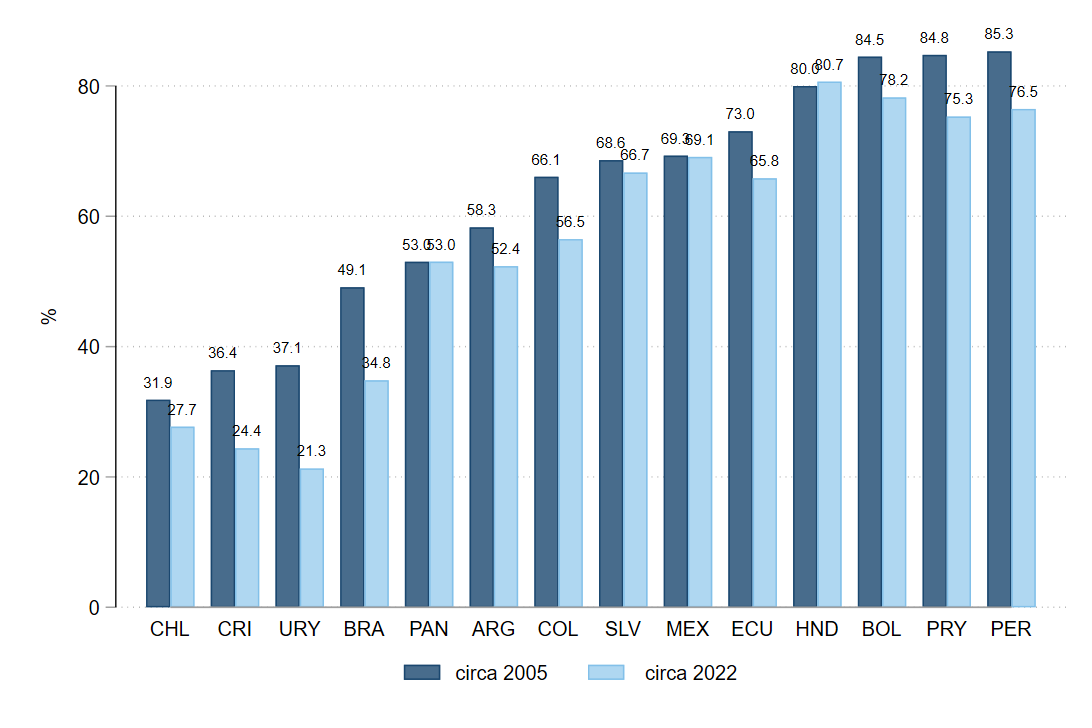
\includegraphics[width=0.5\linewidth]{latex/figures/Snapshot/snapshot_informal_ss.png}
    \label{fig:SalariedSS}
    \footnotesize{Source: Household Surveys-SEDLAC.}
    \footnotesize{Note: Each bar is a weighted average of each country, weighting by total workers in 2005 and 2021.  Data corresponds to 2021 except for Chile 2022, Guatemala 2014; Honduras 2019; Mexico 2018 and Uruguay 2019.}
\end{figure}
    
\end{frame}

%---------------------------------------------------------

%---------------------------------------------------------

\begin{frame}
\frametitle{Changes over time}
\begin{figure}[!htb]
    \justifying
     \caption{Salaried who do not contribute to SS}     
       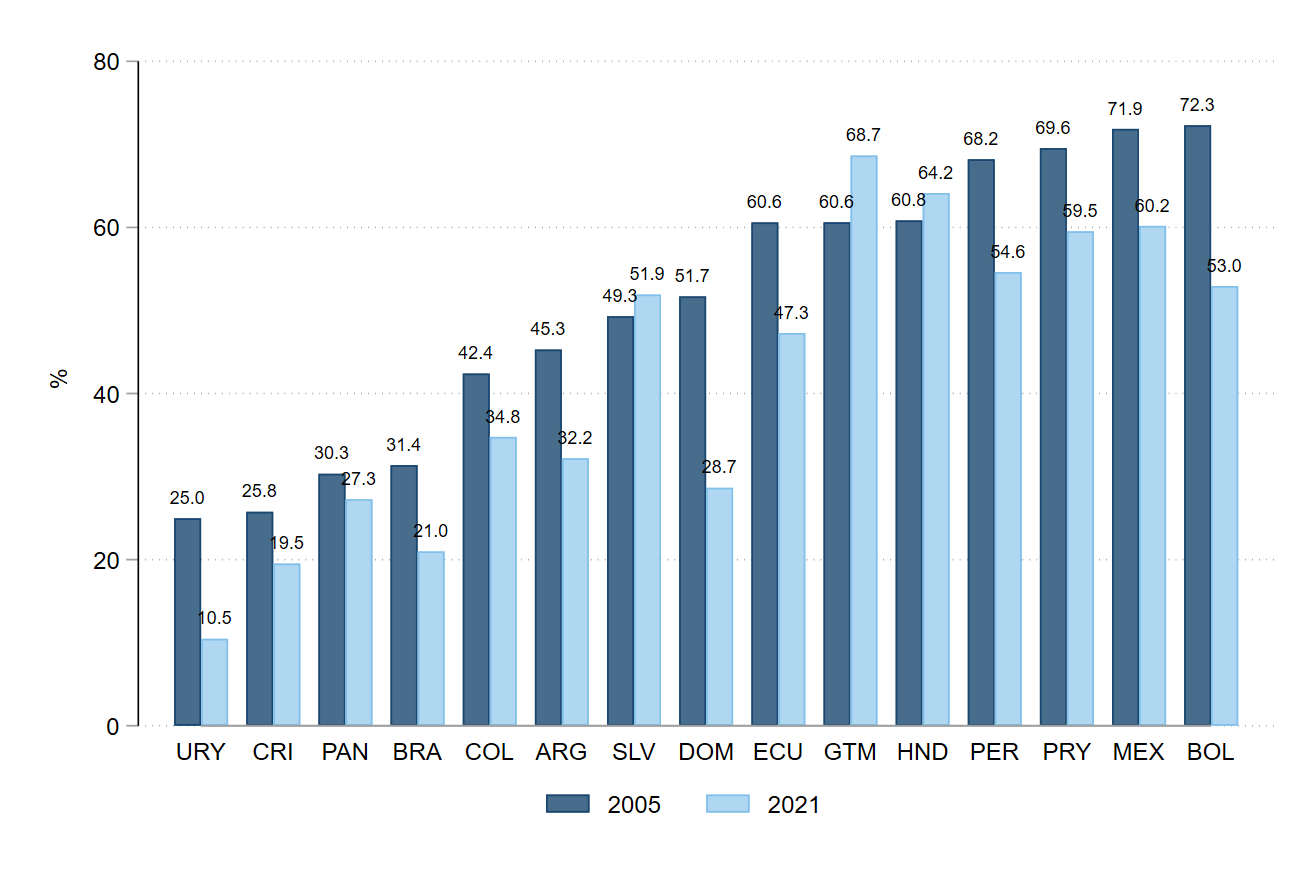
\includegraphics[width=0.5\linewidth]
       {latex/figures/Snapshot/snapshot_informal_ss_dep.png}
    \label{fig:SalariedSS}
    \footnotesize{Source: Household Surveys-SEDLAC.}
    \footnotesize{Note: Each bar is a weighted average of each country, weighting by total workers in 2005 and 2021.  Data corresponds to 2021 except for Chile 2022, Guatemala 2014; Honduras 2019; Mexico 2018 and Uruguay 2019.}
\end{figure}


    
\end{frame}

%---------------------------------------------------------

\begin{frame}
\frametitle{Changes over time}
\begin{figure}[!htb]
    \justifying
     \caption{Salaried who work at small firms}     
     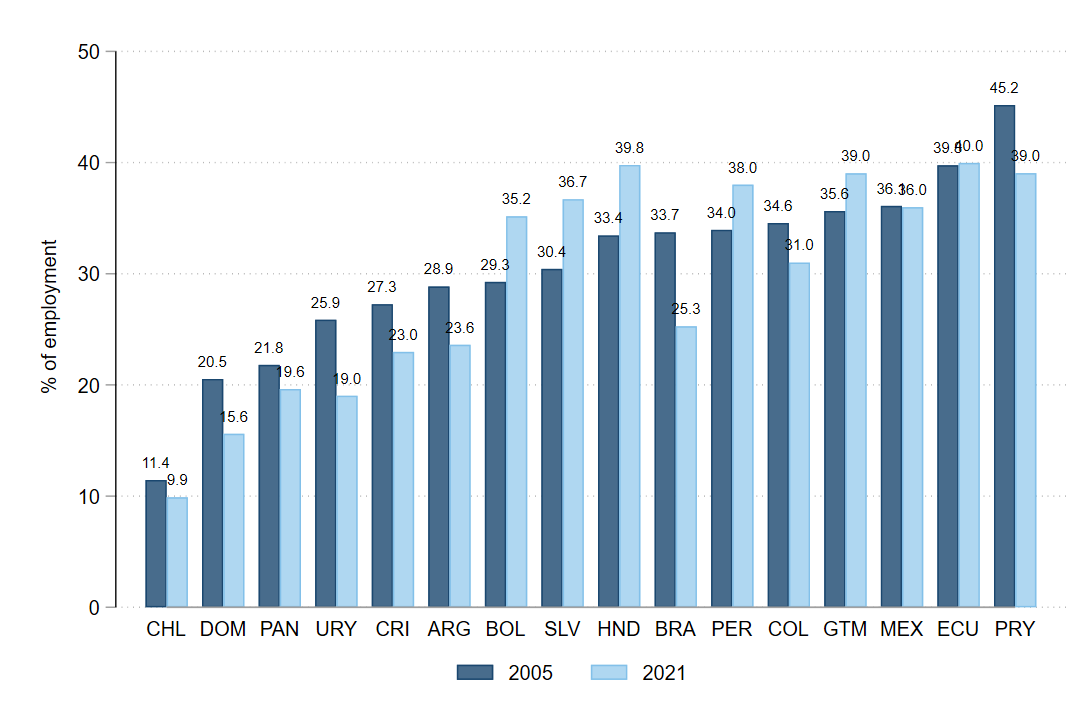
\includegraphics[width=0.5\linewidth]{latex/figures/Snapshot/snapshot_dependents_small.png}
    \label{fig:SalariedSmall}
    \footnotesize{Source: Household Surveys-SEDLAC.}
    \footnotesize{Note: Each bar is a weighted average of each country, weighting by total workers in 2005 and 2021.  Data corresponds to 2021 except for Chile 2022, Guatemala 2014; Honduras 2019; Mexico 2018 and Uruguay 2019.}
\end{figure}
\end{frame}
%---------------------------------------------------------
%Example of the \pause command
\begin{frame}
In this slide \pause

the text will be partially visible \pause

And finally everything will be there
\end{frame}
%---------------------------------------------------------

\section{Regional heterogeneity}

%---------------------------------------------------------
%Highlighting text
\begin{frame}
\frametitle{Informality in LAC}

In this slide, some important text will be
\alert{highlighted} because it's important.
Please, don't abuse it.

\begin{block}{Remark}
Sample text
\end{block}

\begin{alertblock}{Important theorem}
Sample text in red box
\end{alertblock}

\begin{examples}
Sample text in green box. The title of the block is ``Examples".
\end{examples}
\end{frame}
%---------------------------------------------------------


%---------------------------------------------------------
%Two columns
\begin{frame}
\frametitle{Two-column slide}

\begin{columns}

\column{0.5\textwidth}
This is a text in first column.
$$E=mc^2$$
\begin{itemize}
\item First item
\item Second item
\end{itemize}

\column{0.5\textwidth}
This text will be in the second column
and on a second tought this is a nice looking
layout in some cases.
\end{columns}
\end{frame}
%---------------------------------------------------------


\end{document}